\documentclass{article}
\usepackage[utf8]{inputenc}
% Paper settings:
\usepackage[a4paper, margin=3cm]{geometry}
\usepackage{fancyhdr}
\usepackage{enumitem}
\usepackage{changepage}
\usepackage{lastpage}
\usepackage{graphicx}

\title{\line(1,0){400}\\ \textbf{Informatics 2B - Coursework 2} \\ Task 2 - k-NN and Gaussian Classification\\\line(1,0){400}}
\author{s1765026 - University of Edinburgh}
\date{April 2019}

% Setting up header and footer:
\pagestyle{fancy}
\fancyhf{}
\makeatletter
\let\thetitle\@title
\let\theauthor\@author
\makeatother
\lhead{\theauthor}
\rhead{Informatics 2B - Coursework 2}
\cfoot{\thepage /\pageref{LastPage}}

\setlength{\parskip}{5pt}
\setlength{\parindent}{0pt}

% ----------- preamble over -----------------

\begin{document}

\maketitle
\thispagestyle{empty} % removes page number

\newpage
\pagenumbering{arabic} % start page numbering here

%-----------Start of task 1 here % -----------

\subsection*{Task 2.1}

\begin{center}
\begin{tabular}{ |c|c|c|c|c|c| } 
 \hline
 K & 1 & 3 & 5 & 10 & 20 \\ 
 \hline
 Runtime (secs) & 32.10 & 32.10 & 32.11 & 32.11 & 32.12 \\
 \hline
 Number of Samples (N) & \multicolumn{5}{|c|}{3998} \\
 \hline
 Number of errors (Nerrs) & 108 & 112 & 124 & 132 & 156 \\
 \hline
 Accuracy (acc) & 97.29865\% & 97.19860\% & 96.89845\% & 96.69835\% & 96.09805\% \\
 \hline
\end{tabular}
\end{center}

The runtimes presented in the table includes the overhead (31.92 secs) of computing the distance and sorting of k-NN. This is only computed once, but if we were running the function for a single value of k the time it would take is approximately what is presented on the table rather than a negligible value (excluding the overhead). That is the reason the decision was made to use such value.

\subsection*{Task 2.2}

To tackle this question we had to reduce the dataset to a conservative size. We choose the first 2000 samples as this is guaranteed to fit in memory of any modern machine. \par
This limitation was imposed by the fact that vectorising the square distance function requires a large amount of memory. In all other parts of the assignment, the memory available is more than enough, but in this case the best we can hope for is to either not vectorise our code, making it very slow, or to use only a subset of the data points, which is what has been done.

\begin{center}
    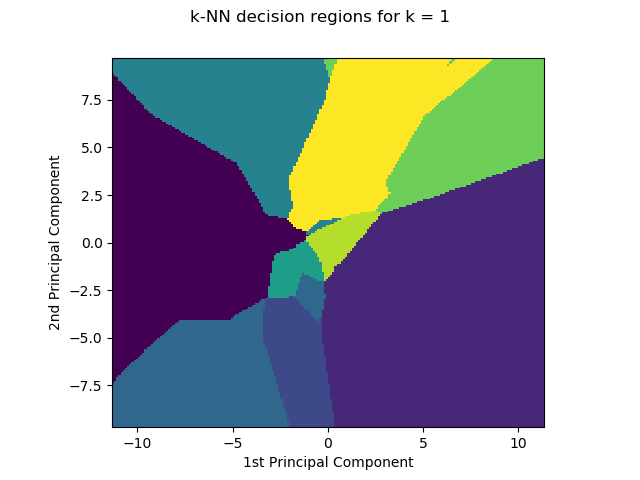
\includegraphics[trim=3cm 0 0 0, scale=0.5]{images/task2_2_imgs_1.png}
    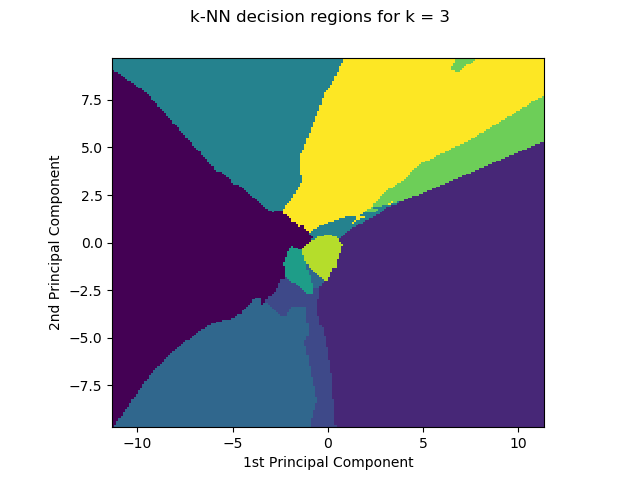
\includegraphics[trim=0 0 3cm 0, scale=0.5]{images/task2_2_imgs_3.png}
\end{center}


\newpage

\subsection*{Task 2.3}

\begin{center}
    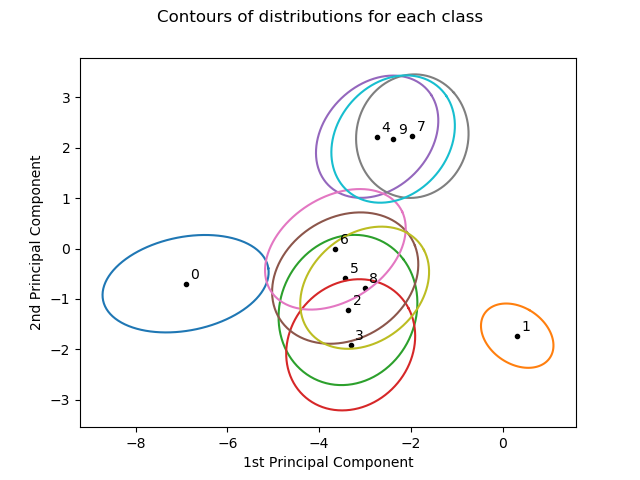
\includegraphics[trim=0 0 0 0, scale=0.55]{images/task2_3_img.png}
\end{center}

\subsection*{Task 2.4}

\begin{tabular}{ |c|c| } 
    \hline
    K & Correlation ($r_{12}$) \\ 
    \hline
   1 & -0.20890 \\
    \hline
   2 & 0.15840  \\
    \hline
   3 & 0.06222  \\
    \hline
   4 & -0.43908 \\
    \hline
   5 & 0.59212 \\
    \hline
   6 & -0.31049 \\
    \hline
   7 & 0.31548 \\
    \hline
   8 & 0.54231 \\
    \hline
   9 & 0.11689 \\
    \hline
   10 & 0.44342 \\
    \hline
   All & $7.78629 \times 10^{-17}$ \\
    \hline
\end{tabular}


% \begin{tabular}{ |c|c|c|c|c|c| } 
%     \hline
%     K & 1 & 2 & 3 & 4 & 5 \\ 
%     \hline
%     Correlation ($r_{12}$) & -0.20890 & 0.15840 & 0.06222 & -0.43908 & 0.59212 \\
%     \hline
% \end{tabular}
% \vspace{0.5cm}
% \\
% \begin{tabular}{ |c|c|c|c|c|c| } 
%      \hline
%      K & 6 & 7 & 8 & 9 & 10 \\ 
%      \hline
%      Correlation ($r_{12}$) & -0.31049 & 0.31548 & 0.54231 & 0.11689 & 0.44342 \\
%      \hline
% \end{tabular}
% \vspace{0.5cm}
% \\
% \textbf{Overall Correlation: $7.78629 \times 10^{-17}$} 

\subsection*{Task 2.5}

\begin{tabular}{ |c|c| } 
 \hline
 Runtime (secs) & 2.5 \\
 \hline
 Number of Samples (N) & 3998 \\
 \hline
 Number of errors (Nerrs) & 199 \\
 \hline
 Accuracy (acc) & 95.02251\% \\
 \hline
\end{tabular}

\newpage
\subsection*{Task 2.6}

\begin{center}
    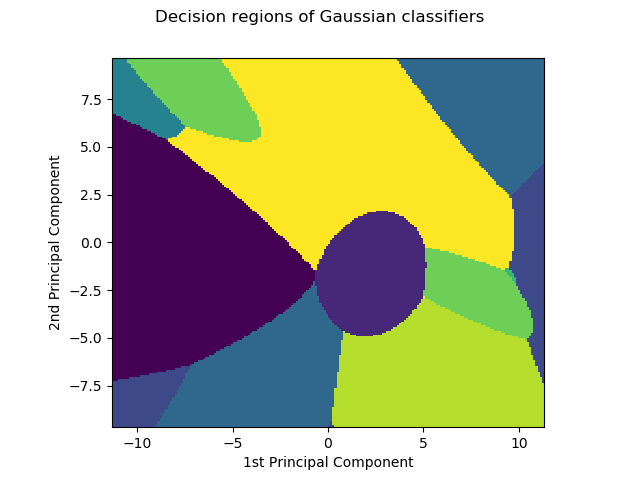
\includegraphics[trim=0 0 0 0, scale=0.6]{images/task2_6_img.png}
\end{center}


\subsection*{Task 2.7}
\begin{center}
\begin{tabular}{ |c|c|c|c|c|c|c|c| } 
    \hline
    Ratio & 0.9 & 0.8 & 0.7 & 0.6 & 0.5 & 0.4 & 0.3 \\ 
    \hline
    Accuracy & 94.9725\% & 94.9725\% & 94.9975\% & 95.2226\% & 95.0725\% & 94.9475\% & 95.1476\% \\
    \hline
\end{tabular}
\end{center}

\subsection*{Task 2.8}

\begin{center}
\begin{tabular}{ |c|c|c|c| } 
 \hline
 L & 2 & 5 & 10 \\ 
 \hline
 Runtime (secs) & 7.07 & 15.99 & 26.01 \\
 \hline
 Number of Samples (N) & \multicolumn{3}{|c|}{3998} \\
 \hline
 Number of errors (Nerrs) & 175 & 121 & 93 \\
 \hline
 Accuracy (acc) & 95.62281\% & 96.97349\% & 97.67384\% \\
 \hline
\end{tabular}
\end{center}


%-------------- End of task 1 % ------------

\end{document}
